\chapter{Related work}
\label{sec:related_work}
This chapter provides overview of the existing methods that are directly related to the topic of the thesis. This includes techniques for malicious URL detection based on generalizable string information and methods for model compression.

\section{Manual Feature Engineering}
\label{sec:man_feat_eng}
One of the simplest approaches to malicious URL detection is to extract a set of manually engineered features from the URL string and train a standard feature-based classifier. This strategy is followed in~\cite{lexicalFeaturesModels}, and a broader overview of such features is presented in the survey by~\cite{surveymaliciousfeatures}.

Features that these papers mention can be summarized as follows:
\begin{itemize}
    \item \textbf{From the whole URL} -- length; the number of semicolons, underscores, question marks, equals, ampersands; digit to letter ratio; entropy of the string
    \item \textbf{SLD} -- contains IP; length; number of digits; number of non-alphanumeric characters; number of hyphens; number of @s
    \item \textbf{TLD} -- presence in suspicious list
    \item \textbf{Subdomain} -- number of dots; number of subdomains
    \item \textbf{Path} -- number of '//'; number of subdirectories; presence of '\%20'; presence of uppercase directories; presence of single-character directories; number of special characters; number of zeroes; ratio of uppercase to lowercase characters
    \item \textbf{Query parameters} -- total length; number of queries; number of variables; presence of encoded scripts (e.g., Base64)
    \item Presence of specific \textbf{keywords} -- (e.g., \texttt{login}, \texttt{secure}, \texttt{cmd=}, \texttt{redirect=}, \texttt{confirm}, \texttt{update}, \texttt{verify}, \texttt{account})
\end{itemize}

These features are extracted using a combination of URL parsing, regular expressions, and custom logic. Once extracted, they are fed into a classifier. In~\cite{lexicalFeaturesModels}, models such as logistic regression, XGBoost, and Naive Bayes were used.

No single feature is sufficient to identify a malicious URL definitively. Therefore, implementing a lightweight rule-based system (e.g., using regexes) to pre-filter URLs before the main classifier and gain speedup would degrade predictive performance significantly.

The main advantages of feature-based models are that they are computationally efficient, easy to train and highly interpretable. However, the attackers can adapt their URLs to evade detection by modifying the URL structure or using obfuscation techniques that the features do not cover. This generalization problem is obvious in the keywords features, where the model is trained on a specific set of keywords, and when new keywords appear, or their obfuscated versions are used, the model fails to detect them. This drives the need for more generalizable models based on deep learning.

Nevertheless, the rise of deep learning models does not invalidate the utility of handcrafted features. Certain information, such as URL length, frequency of characters, or the structure of components, is often better represented explicitly. A hybrid approach can be beneficial, where handcrafted features are combined with outputs from a deep learning model. One common strategy is to use the output of the deep model as an input feature for a traditional classifier, a technique known as stacking.

\section{Deep learning-based models}
\label{sec:dl_models}
Unlike feature-based models, the input to deep learning models is the raw URL string. The model learns to extract relevant features from the data during training. This approach allows model to learn more generalizable features, which are not easily captured by handcrafted features, especially in the interaction of semantic and syntactic information.

One of the earliest deep learning models designed specifically for URL-based malicious detection is URLNet~\cite{URLNet}. It uses a dual-branch convolutional neural network (CNN) architecture: one branch processes the URL at the character level and the other at the word level. The character-level branch focuses on patterns such as obfuscation through character substitutions, while the word-level branch targets higher-level structural and semantic patterns by embedding words that are extracted using delimiters like dots or slashes. Both branches are trained jointly in an end-to-end fashion, and their outputs are concatenated and passed through fully connected layers for final classification.

Another example would be a model from GramBeddings~\cite{GramBeddings} paper. Aside from the model, the paper also introduces a new dataset, which is also used in this thesis for experiments. Its description is provided in the dataset Section~\ref{sec:dataset_descriptions}. The model learns embeddings for the most common n-grams (group of n consecutive characters), which are chosen based on dataset statistics and then uses CNN, LSTM (Long short-term memory) and attention mechanisms for classification. Multiple values of $n$ are used to capture different ranges of local context.

Many other deep learning-based models have been proposed, however, they were all recently overshadowed by transformer-based models, therefore other non-transformer models are not discussed in detail.

\section{Transformer-based models}
Transformer-based~\cite{AttentionIsAllYouNeed} models have achieved state-of-the-art results in many natural language processing tasks, including malicious URL detection.

\subsection{BERT}
As demonstrated by the 2021 paper URLTran,~\cite{URLTran}, fine-tuning encoder transformers like BERT~\cite{BERT} or RoBERTa~\cite{RoBERTa} on URL classification tasks has proven very effective.

Before running the model, the input text is tokenized using WordPiece~\cite{wordpiece} tokenizer, which splits words into subword units. This allows the model to handle out-of-vocabulary words and reduces the vocabulary size. The tokenizer also adds special tokens to the input sequence, such as [CLS] for the classification of the whole sentence and [SEP] for segment separation.

The input to BERT is a sequence of tokens formatted as:
$$
    \text{[CLS]},\ t_1,\ t_2,\ \dots,\ t_n,\ \text{[SEP]}
$$
Where [CLS] is a special classification token, and [SEP] marks the end of a single sentence or separates two segments.

Unlike traditional unidirectional models, BERT is bidirectional -- it learns contextual representations by attending to both the left and right of every token at every layer. Since the task of malicious URL only only requires classification, not generation, encoder only models are sufficient.

For example, consider the URL example from~\cite{URLTran}:

\begin{table}[H]
    \centering
    \renewcommand{\arraystretch}{1}
    \resizebox{\textwidth}{!}{
        \begin{tabular}{ll}
            \toprule
            \textbf{Original URL}       & \texttt{secure.bankofamerica.com/login/sign-in/signOnV2Screen.go}                                                                                                                \\
            \midrule
            \textbf{Tokenized Sequence} &
            \texttt{[CLS]}, \texttt{secure}, \texttt{.}, \texttt{bank}, \texttt{\#\#of}, \texttt{\#\#ame}, \texttt{\#\#rica}, \texttt{.}, \texttt{com}, \texttt{/}, \texttt{log}, \texttt{\#\#in}, \texttt{/},             \\
                                        & \texttt{sign}, \texttt{-}, \texttt{in}, \texttt{/}, \texttt{sign}, \texttt{\#\#on}, \texttt{\#\#v}, \texttt{\#\#2}, \texttt{\#\#screen}, \texttt{.}, \texttt{go}, \texttt{[SEP]} \\
            \bottomrule
        \end{tabular}}
    \caption{Example of WordPiece tokenization applied to a URL.}
    \label{tab:tokenization_example}

\end{table}

The tokens are converted to embedding vectors using a learned embedding matrix. Learned positional embeddings can be added~\cite{AttentionIsAllYouNeed} because transformer architecture is permutation invariant.

These embeddings are then fed into the BERT model, whose architecture can be seen in Figure~\ref{fig:transformer}.

\begin{figure}[H]
    \centering
    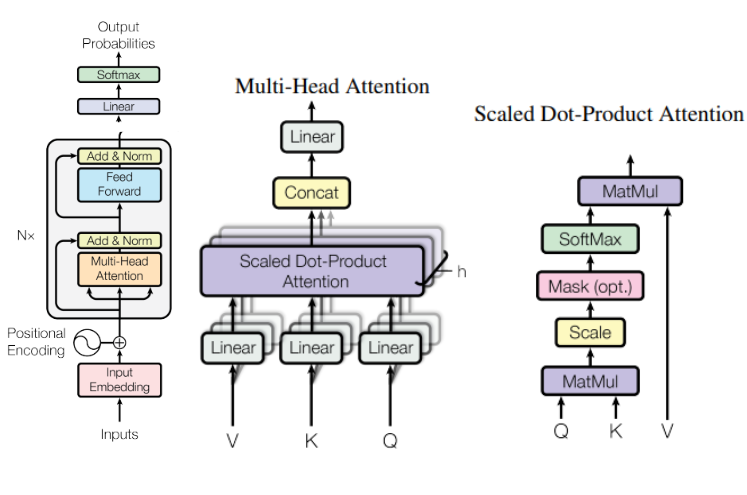
\includegraphics[width=0.9\textwidth]{images/transformer.png}
    \caption{Illustration of an encoder-only transformer architecture. Images are from~\cite{AttentionIsAllYouNeed}. On the left, the entire transformer architecture is shown. In the middle, a multi-head attention block on the left is shown. On the right, scaled-dot-product attention from the middle image is described in detail.}
    \label{fig:transformer}
\end{figure}

It consists of a stack of $N$ identical encoder layers, each containing two main components: a multi-head self-attention mechanism and a feed-forward neural network. Each of these components is followed by layer normalization and residual connections. The input to the scaled-dot-product is a tensor of shape \textit{(batch\_size, sequence\_length, embedding\_dimension)} obtained by multiplying previous layer representations by learned attention matrices. The output is a tensor of the same shape, which is then passed to the feed-forward network.

The self-attention layer provides contextual information to individual token embeddings, and the feed-forward network applies a non-linear transformation to the output of the self-attention layer. More on how the transformers work can be found in~\cite{AttentionIsAllYouNeed,RoBERTa}.

The output used for classification of malicious URLs is then obtained by taking the embedding of the [CLS] token from the last layer of the transformer and passing it through a linear layer with softmax activation function. The output is a probability distribution over the classes, which can be interpreted as the model's confidence in each class.

\subsection{Training strategies}
The models used in URLTran~\cite{URLTran} use pre-trained BERT and RoBERTa models, which are fine-tuned on the target task. The pre-training process involves training the model on a large corpus of text using two tasks: masked language modelling (MLM) and next sentence prediction (NSP).

This allows the model to use semantic knowledge about the keywords in the URL. By fine-tuning the model on the URL dataset, it then strives to learn the specific patterns unique to URLs.

The model can also be pre-trained directly on the URL corpus. This approach is used, for example, by~\cite{urlbert}. The positive aspect of this approach is that the model learns potentially better tokenization for the URL strings, which can be beneficial for the task. On the other hand, it loses the general knowledge about the language, which can be useful for the task because of the presence of specific keywords in the URLs, as mentioned earlier.

Different data augmentation techniques are mentioned in~\cite{URLTran} to learn specific types of attacks. This way, the dataset size can be artificially increased. The first technique is parameter reordering. The second focuses on splitting domain names into words and inserting hyphen characters in between them. The third technique tries to target homoglyph attacks by replacing characters with similar-looking ones.

\subsection{Other architecture improvements}
This sub-section outlines approaches that are not used in this thesis but are proposed as potential directions for future work.

Improvements to the original BERT architecture have been proposed, one of the most notable being CharBERT~\cite{charbert}. This model combines standard subword-level embeddings with additional character-level information using a bidirectional GRU, fusing both representations. Since malicious URLs often vary at the character level, this method may provide valuable information.

One paper applying this idea to malicious URL detection is~\cite{TransURL}, which builds on CharBERT and introduces several enhancements. Although it claims state-of-the-art results, the paper lacks direct comparison with other transformer-based models and uses an evaluation protocol susceptible to domain over-fitting (as discussed in the dataset chapter). A reevaluation of the model would be necessary, and if it proves superior to standard BERT, model distillation could be a promising next step to improve the speed-quality trade-off.

\section{Methods for model compression}
\label{sec:model_compression_methods}

This chapter explores the second approach to improving the speed-quality ratio mentioned in the introductory chapter. Rather than selecting a smaller model from the beginning, this approach focuses on transforming a larger model into a faster version by using model compression methods.

Several existing methods are presented in terms of how they work and how they can be implemented. A brief discussion is included for each method to justify its use or omission in the experimental work.

\subsection{Quantization}

Quantization is a concept that extends beyond the field of machine learning. It generally refers to the process of mapping a large set of input values to a smaller, discrete set.

In the context of machine learning, the purpose of quantization is to map values needed to perform operations of the model from high-precision format (e.g., Float32~\cite{ieee754}) to lower-precision format (e.g., Int8, Float16). The operation is then performed using the lower-precision format, which is faster (if the target hardware supports it) and requires less memory both at runtime and for storing the model. The information from these sources was used for writing this Section~\cite{quantization_whitepaper, nvidia_whitepaper}.

To better understand quantization, consider the example of matrix-vector multiplication that is present in most neural networks. The operation can be expressed as:
\begin{equation}
    y = Wa + b
\end{equation}
where $W$ is the weight matrix, $a$ is the input vector, $b$ is the bias vector, and $y$ is the output vector. This operation, such as all other operations in a model, requires two types of values, which need to be quantized in different ways:
\begin{itemize}
    \item \textbf{Weights} -- These are the parameters of the operation learned during training. They are fixed during inference. In this case, $W$ and $b$ are weights.
    \item \textbf{Activations} -- These are the intermediate outputs of the operation, which depend on the input data. They change for each forward pass. In this case, $a$ and $y$ are activations.
\end{itemize}

\subsubsection*{Float16 quantization}

Float16 (also known as FP16) is a reduced-precision floating-point format that uses 16 bits to represent numbers. It retains the same structural components as Float32 -- a sign bit, exponent, and mantissa, but with fewer bits: 1 for a sign, 5 for the exponent, and 10 for the mantissa. This makes it more memory -- and compute-efficient than Float32 while still being capable of representing a wide dynamic range.

Unlike Int8 quantization, which requires all values to be mapped into a fixed integer range, Float16 quantization allows dynamic range representation because of the ability of floating-point numbers of use exponent to represent both very small and very large numbers.

When quantizing to Float16, the only thing that needs to be done is therefore a simple conversion of the Float32. The model then can use Float16 at runtime instead of Float32 without any additional changes.

\subsubsection*{Int8 quantization}

Unlike the previous example, Int8 quantization requires a more complex process. The goal is to map the original float values to a smaller fixed integer range, typically from -128 to 127 for signed integers. The mapping is typically done for each tensor separately. Alternative approach are to quantize by parts of the tensor, for example by rows.

The especially problematic part is that the Float32 tensor can have a very wide range of values, while the Int8 representation can only represent 256 discrete values. This means that the quantization process must carefully choose how to map the float values to the Int8 range. If done poorly, the majority of values in the tensor may be mapped outside of this range and clipped, or in the other case, the majority of values may be mapped to a single value, losing important information.

The quantization process can be expressed mathematically as follows:

\begin{equation}
    q = \text{round}\left(\frac{x}{s}\right) + z
    \label{eq:quantize}
\end{equation}
\begin{equation}
    \hat{x} = s \cdot (q - z)
    \label{eq:dequantize}
\end{equation}

Here:
\begin{itemize}
    \item $x$ is the original float value,
    \item $q$ is the quantized integer value,
    \item $s$ is the scale factor (a positive real number),
    \item $z$ is the zero-point (an integer that aligns 0 in float to an integer in the quantized domain).
\end{itemize}

Based on choosing the values of $z$, there are two main strategies. The first one is asymmetric quantization, which allows the zero-point $z$ to be non-zero, which is helpful for values that do not centre around, especially activations.

The second one is symmetric quantization, which assumes that the float range is symmetric around zero. In this case, $z = 0$, and only the scale $s$ needs to be calculated. This is much more efficient as described in~\cite{nvidia_whitepaper}. Often, accelerators support only this type of quantization.

\subsubsection*{Static vs. dynamic quantization}

The weights of the model are static and do not change during inference. Therefore, the quantization coefficients can be computed offline and also remain unchanged, since the range of tensors is known ahead of time.

That is not the case for activations, which are dependent on the input tensor. There are two main strategies for computing these parameters for activations: static and dynamic quantization. The difference between them lies in \textbf{when} the quantization parameters ($s$, $z$) are calculated and \textbf{what data} is used to compute them.

\textbf{Static quantization} computes scale and zero-point values ahead of time before inference. This is done using a calibration dataset, which is a representative subset of the training or validation data. The quantization parameters are derived from the observed distributions of activations and remain fixed during inference. Because these parameters are known in advance, static quantization allows for faster inference.

The simplest approach for computing the scale and zero-point is based on the minimum and maximum values of the activation or weight tensor:
$$
    s = \frac{x_{\text{max}} - x_{\text{min}}}{q_{\text{max}} - q_{\text{min}}}, \quad z = \text{round}\left(q_{\text{min}} - \frac{x_{\text{min}}}{s}\right)
$$
However, this \textbf{min-max} method is sensitive to outliers, which can lead to overly large quantization ranges and poor resolution for most values.

To address this, more sophisticated strategies are often used:

\begin{itemize}
    \item \textbf{Percentile-based calibration} clips the extreme values and uses a predefined percentile range (e.g., 99.9\%) to compute $x_{\text{min}}$ and $x_{\text{max}}$. This improves precision by ignoring rare outliers.
    \item \textbf{Entropy-based calibration} selects the quantization range that minimizes the Kullback-Leibler divergence between the original (float) distribution and the quantized distribution.
    \item \textbf{MSE-based calibration} minimizes the mean squared error between the original and quantized tensors.
\end{itemize}

\textbf{Dynamic quantization}, on the other hand, computes quantization parameters on-the-fly during inference. Only weights are quantized offline. When activations are encountered during inference, their scale and zero-point are computed based on the actual input batch.

\subsubsection*{Post-training quantization vs. quantization-aware training}

Once the quantization scheme is chosen, the quantized model can be obtained either through post-processing or during training.

\textbf{Post-training quantization (PTQ)} applies quantization after the model has been fully trained. The model's weights and (optionally) activations are quantized, either statically or dynamically. This approach is fast and easy to apply but may lead to reduced predictive performance.

\textbf{Quantization-aware training (QAT)} addresses this by simulating quantization during training. Fake quantization operators are inserted into the computation graph, allowing the model to adapt to quantization noise. This typically results in higher predictive performance, as the model learns to be robust to low-precision representations. However, QAT requires retraining and is more computationally expensive.